\documentclass[a4paper]{article}
\def\DOCTITLE{CSC3424 Bio Algorithms}
% Set document attributes
\title{\DOCTITLE}

\usepackage{fullpage}
\usepackage{scrextend}
\usepackage{titlesec}
\usepackage{fancyhdr}
\usepackage{amsmath}
\usepackage{amssymb}

% Handle graphics correctly
\ifx\pdftexversion\undefined
\usepackage{graphicx}
% \usepackage[dvips]{graphicx}
\else
\usepackage[pdftex]{graphicx}
\DeclareGraphicsRule{*}{mps}{*}{}
\fi

% Setup headers and footers
\pagestyle{fancy}
\lhead{}
\chead{\DOCTITLE}
\rhead{}
\rfoot{}
\cfoot{\thepage}
\lfoot{}

% New page for each section
% \newcommand{\sectionbreak}{\clearpage}

% Set header and footer sizes
\renewcommand{\headrulewidth}{0.4pt}
\renewcommand{\footrulewidth}{0.4pt}
\setlength{\headheight}{15.2pt}
\setlength{\headsep}{15.2pt}

\setlength{\parskip}{5pt plus 1pt minus 1pt}
\setlength{\parindent}{0pt}

\newcommand{\Forall}{\;\forall\;}
\newcommand{\Mod}{\: mod \:}


\begin{document}

\tableofcontents

\section{Cell and Molecular biology}

\subsection{The Cell}

\begin{itemize}
  \item Minimal unit of life
  \item Cell is a system of many components enclosed in a series of membranes
  \item Small organisms such as fungi and bacteria are unicellular
  \item Plants and animals are generally multicellular
\end{itemize}

\subsubsection{Prokaryotes}

\begin{itemize}
  \item All prokaryotes are single cell
  \item Smaller than eukaryotic cells \\
        ($< 1 \mu \mathrm{m}$ in diameter)
  \item Simple structure \\
        No inner cellular membranes
  \item Very adaptable to environment \\
        Found in almost every habitat
  \item Approximately $5x10^{30}$ prokaryotic cells in the world
  \item Essential for healthy life
\end{itemize}

\Para{Prokaryotic cell}

\begin{itemize}
  \item Less complex than eukaryotic cells
  \item Contain no organelles
  \item Believed to represent the earliest life on earth and that eukaryotic
        cells evolved from prokaryotic cells
\end{itemize}

\begin{figure}[h!]
  \centering
  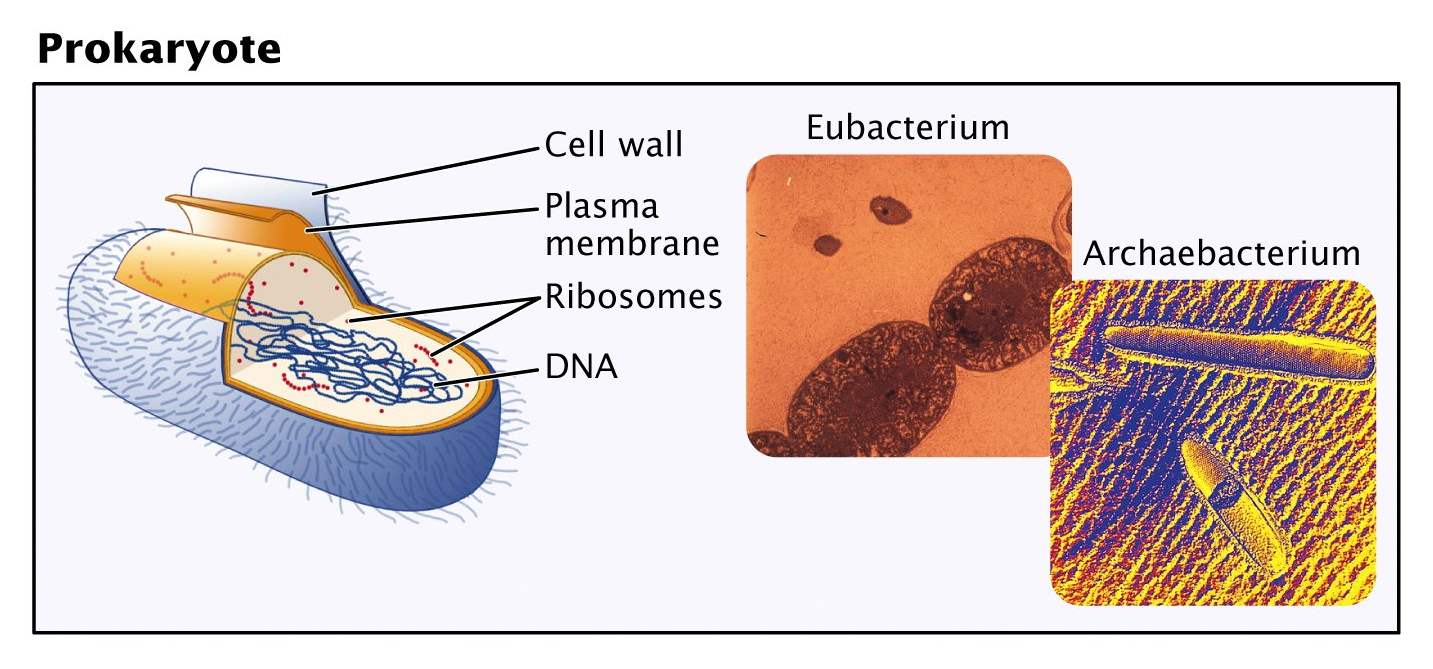
\includegraphics[width=0.7\textwidth]{graphics/prokaryotic_cell.eps}
  \caption{Prokaryotic cell structure}
  \label{fig:prokaryotic_cell}
\end{figure}
\FloatBarrier

\Para{Types of prokaryotes}

Types descend from common ancestor.

\begin{description}
  \item[Eubacteria] \hfill \\
    Common bacteria that affects life daily
  \item[Archaea] \hfill \\
    Tend to exist in extreme habitats (high pressure, temperature, pH)
\end{description}

\subsubsection{Eukaryotes}

\begin{itemize}
  \item More structurally and biochemically complex than prokaryotes
  \item Evolutionarily more recent
  \item Believed to have evolved through endosymbiosis
\end{itemize}

\begin{figure}[h!]
  \centering
  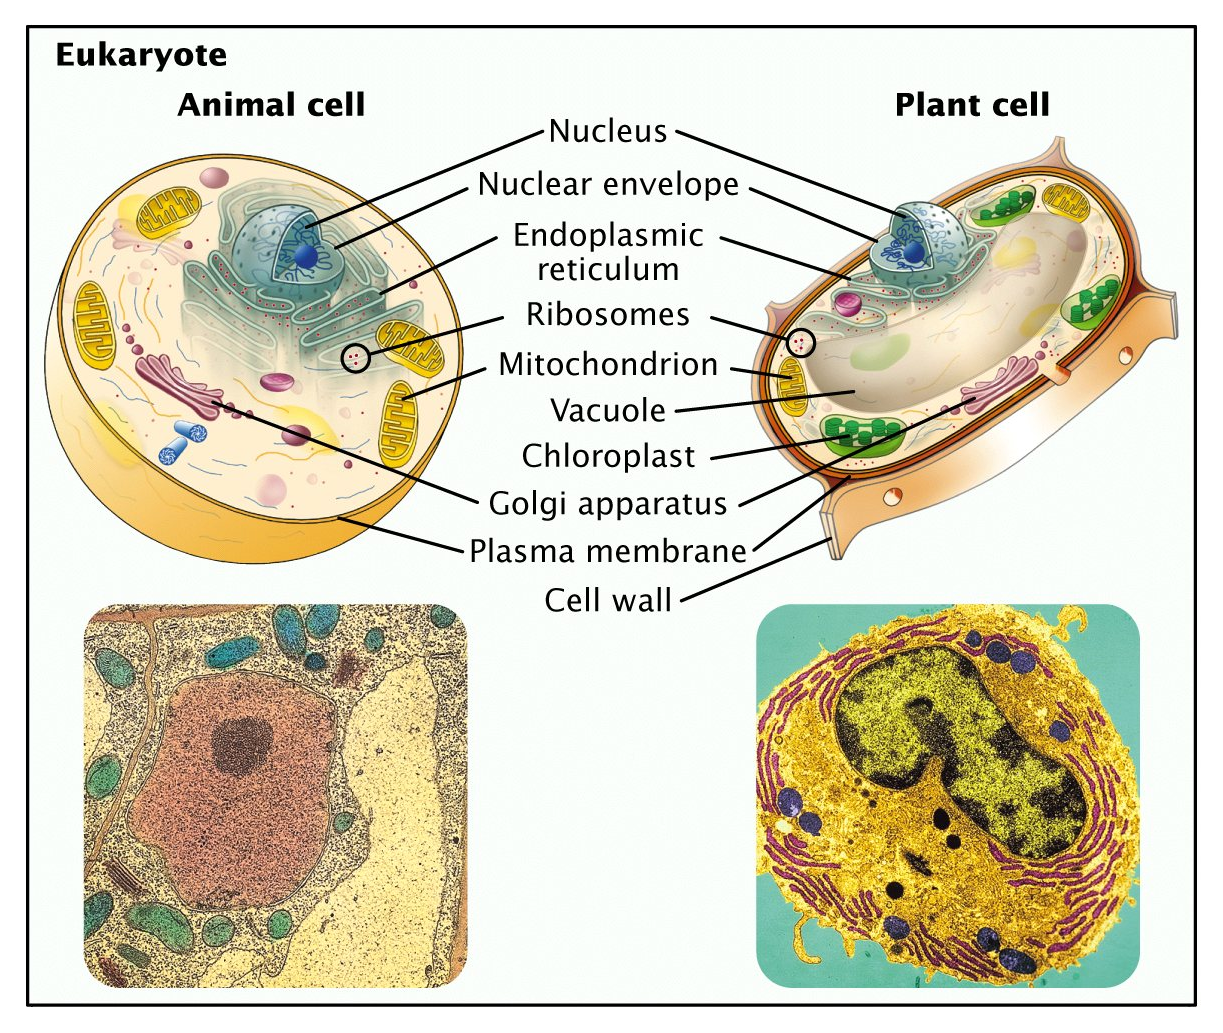
\includegraphics[width=0.7\textwidth]{graphics/eukaryotic_cell.eps}
  \caption{Eukaryotic cell structure}
  \label{fig:eukaryotic_cell}
\end{figure}
\FloatBarrier

\Para{Endosymbiosis}

\begin{itemize}
  \item An ancestral cell engulfed a smaller microbe which continued to survive
        inside it
  \item Both host and prey adapt to new environment and become mutually
        interdependent
\end{itemize}

\subsubsection{Cell functions}

Functions of cells provided by organelle.

\begin{description}
  \item[Nucleus] \hfill \\
    Regulate DNA carrying/replication
  \item[Endoplasmic reticulum] \hfill \\
    System of folded membranes used for transport
  \item[Ribosomes] \hfill \\
    Used to produce proteins
  \item[Mitochondria] \hfill \\
    Provide energy through cellular respiration
  \item[Vacuole] \hfill \\
    Used for storage
  \item[Chloroplasts] \hfill \\
    Used to convert light energy into chemical energy for cell
  \item[Golgi Apparatus] \hfill \\
    Packages and transports proteins
\end{description}

\begin{table}[h!]
  \centering
  \begin{tabular}{@{}lll@{}}
    \toprule
                                & Prokaryotic cells                             & Eukaryotic cells \\
    \midrule
    Nucleus                     & Absent                                        & Present \\
    Cell diameter               & $1-10 \mu \mathrm{m}$                         & $10-100 \mu \mathrm{m}$ \\
    Genome                      & One circular module                           & Multiple linear modules \\
    DNA                         & Not complexed in eubacteria, some in archaea  & Complexed with histomes\\
    DNA quantity                & Small                                         & Large \\
    Membrane-bounded organelles & Absent                                        & Present \\
    Cytoskeleton                & Absent                                        & Present \\
    \bottomrule
  \end{tabular}
  \caption{Comparison of cell types}
  \label{tab:cell_comparison}
\end{table}
\FloatBarrier

\subsubsection{Phenotype from Genotype}

\begin{itemize}
  \item Characteristics of an organism (phenotype) are determined by the
        structure and function of its cells (genotype)
\end{itemize}

\subsection{DNA and genes}

\begin{figure}[h!]
  \centering
  \includegraphics[width=0.2\textwidth]{out/dogma_molecular_biology.eps}
  \caption{Central dogma of molecular biology}
  \label{fig:eukaryotic_cell}
\end{figure}
\FloatBarrier

\subsubsection{Structure of DNA}

\begin{itemize}
  \item Base \\
    Bases bind (A-T, C-G) by Hydrogen bonds
    \begin{itemize}
      \item Pyrimidines
        \begin{itemize}
          \item Cytosine
          \item Thymine
        \end{itemize}
      \item Purines
        \begin{itemize}
          \item Guanine
          \item Adenine
        \end{itemize}
    \end{itemize}
  \item Backbone
    \begin{itemize}
      \item Phosphate \\
        Binds ribose sugar
      \item Ribose sugar \\
        Binds phosphate to base
    \end{itemize}
\end{itemize}

\Para{DNA directionality}

\begin{figure}[h!]
  \centering
  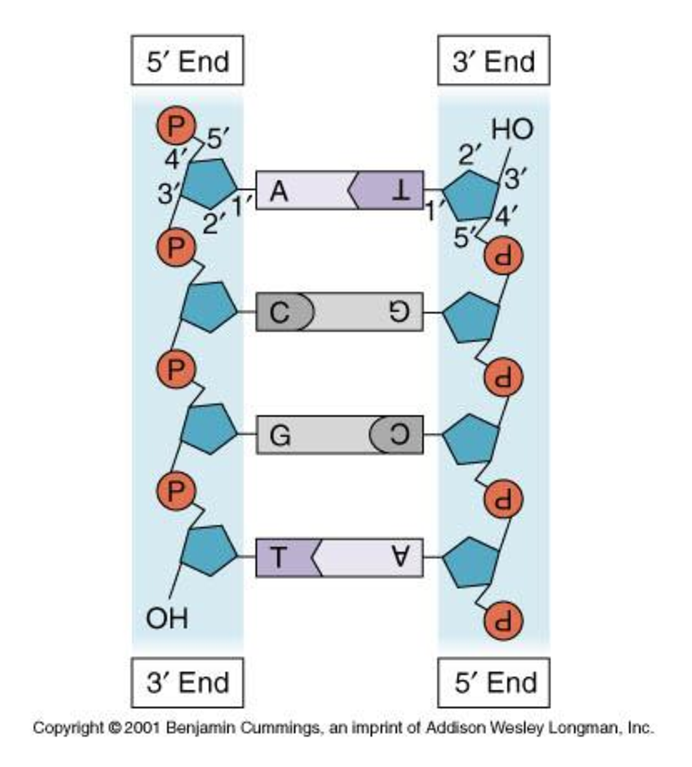
\includegraphics[width=0.4\textwidth]{graphics/dna_directionality.eps}
  \caption{DNA directionality}
  \label{fig:eukaryotic_cell}
\end{figure}
\FloatBarrier

\subsubsection{DNA replication}

\begin{itemize}
  \item Replication is essential for organisms to reproduce
  \item Without replication, cell division could not occur
  \item Replication must be high fidelity but have potential for error (to
        enable evolution)
\end{itemize}

\Para{C-value paradox}

The C-value is the size of an organisms genome (defined as the amount of DNA in
pico grams in a haploid cell).

C-values not reflective of complexity, i.e. no relation between C-value and
number of genes.

\subsubsection{Genome structure}

\Para{Prokaryotic}

\begin{itemize}
  \item Generally small ($<10 \mathrm{M}$ bases)
  \item Single, circular chromosome
  \item Can have plasmids \\
        Disposable genetic elements that often carry genes for antibiotic
        resistance or toxicity
  \item Information dense \\
        Little or no space between genes, genes often overlap
  \item Genes are present in single, uninterrupted units
  \item Multiple genes may be present in single, uninterrupted units
\end{itemize}

\Para{Eukaryotic}

\begin{itemize}
  \item Usually larger than prokaryotic genomes
  \item Multiple, linear chromosomes
  \item Tend to be more information sparse \\
        Large gaps between genes
  \item Genes interrupted by non-coding sequence
    \begin{description}
      \item[Exons] coding
      \item[Introns] non-coding
    \end{description}
\end{itemize}

\subsubsection{DNA packaging}

TODO

\subsection{Transcription}

Process of turning information stored in DNA into RNA.

\begin{description}
  \item[Non-template (coding) strand] \hfill \\
    Contains same base sequence as RNA crated
  \item[Template (non-coding) strand] \hfill \\
    Contains anti-codons of RNA
  \item[Promoter] \hfill \\
    Denotes start of RNA coding region
  \item[Coding region] \hfill \\
    RNA coding
  \item[Terminator] \hfill \\
    DNA coding denoting the end of the coding region
\end{description}

\begin{figure}[h!]
  \centering
  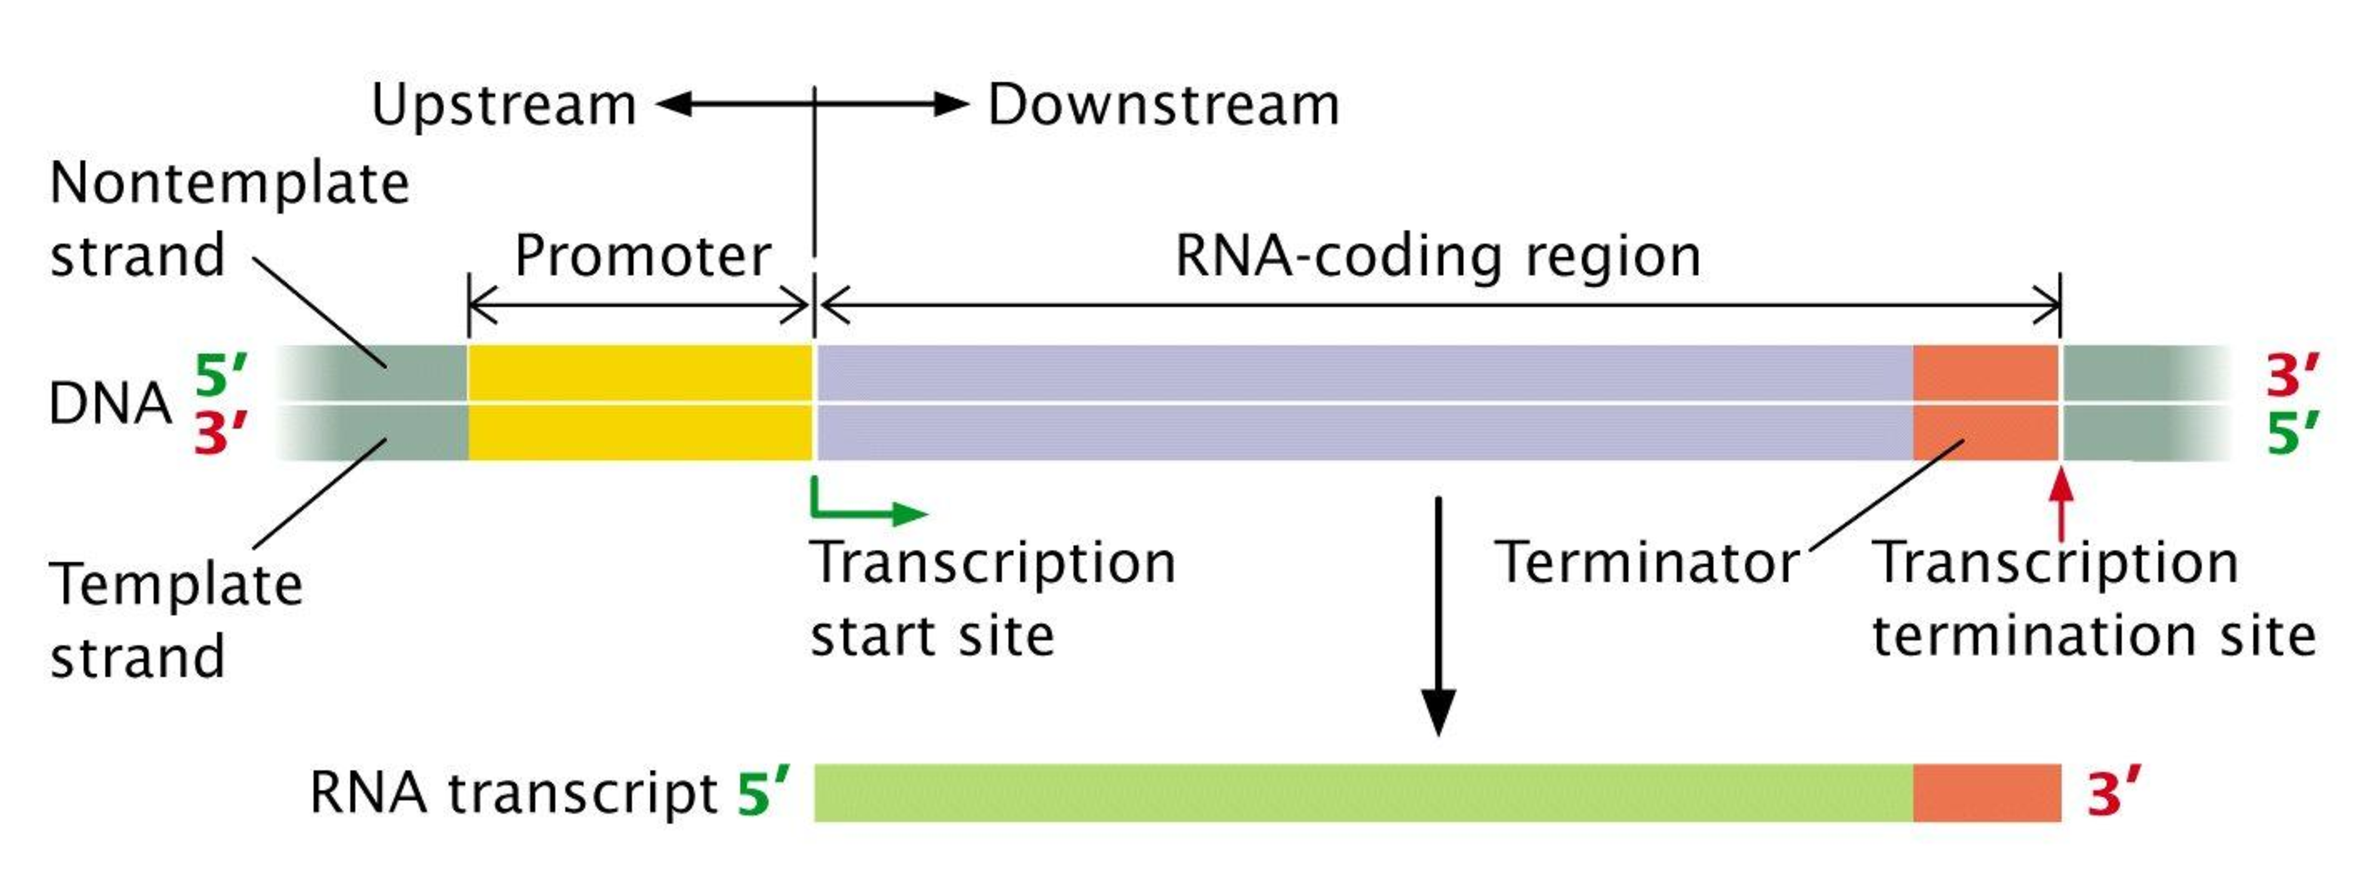
\includegraphics[width=0.8\textwidth]{graphics/dna-rna_transcription.eps}
  \caption{DNA directionality}
  \label{fig:eukaryotic_cell}
\end{figure}
\FloatBarrier

\begin{itemize}
  \item The base Thymine (T) in DNA is replaced with Uracil (U) in RNA
  \item Transcription occurs $5^{\prime}$ to $3^{\prime}$
  \item RNA polymerase is the enzyme responsible for transcription
  \item Transcription in eukaryotes is more complex
\end{itemize}

\subsubsection{Transcript processing}

Primary transcript must be processed into a mature message.

\begin{itemize}
  \item Addition of $5^{\prime}$ cap
    \begin{itemize}
      \item 7-methlyguanosine
      \item Involved in ribosome binding
      \item Protective
    \end{itemize}
  \item $3^{\prime}$ polyadenylation
    \begin{itemize}
      \item Addition of tail of adenosine to mRNA
      \item Required for nuclear export and stability
    \end{itemize}
  \item Splicing
    \begin{itemize}
      \item Primary transcript contains both introns and exons
      \item Introns must be removed
    \end{itemize}
\end{itemize}

\subsection{Translation}

TODO

\section{Genomes and Sequencing}

TODO

\section{Evolution and its effects}

TODO

\section{Transcriptions and Proteomes}

TODO

\end{document}
